\begin{figure*}[h]
\centering
\begin{minipage}{0.45 \textwidth}
\centering
\begin{SQL}[basicstyle=\small, language=HTML]
<fstmt:with target="shown_nations">
SELECT sn.name, (
    SELECT sum(o.total_price) as sumTotal
    FROM db.Orders o, db.Customers c
    WHERE o.cust_ref = c.cust_key
    AND c.nation_ref = sn.nation_key
) as sumTotal
FROM session.SelectedNations sn
</fstmt:with>
<funit:bar_chart>
  <fstmt:for source="shown_nations">
    <column>
      <label> {sn.name} </label>
      <value> {sumTotal} </value>
    </column>
  </fstmt:for>
</funit:bar_chart>
\end{SQL}
\caption{FORWARD Page}
\label{fig:forward-code}
\end{minipage} \hfill
\begin{minipage}{0.45\textwidth}
\centering
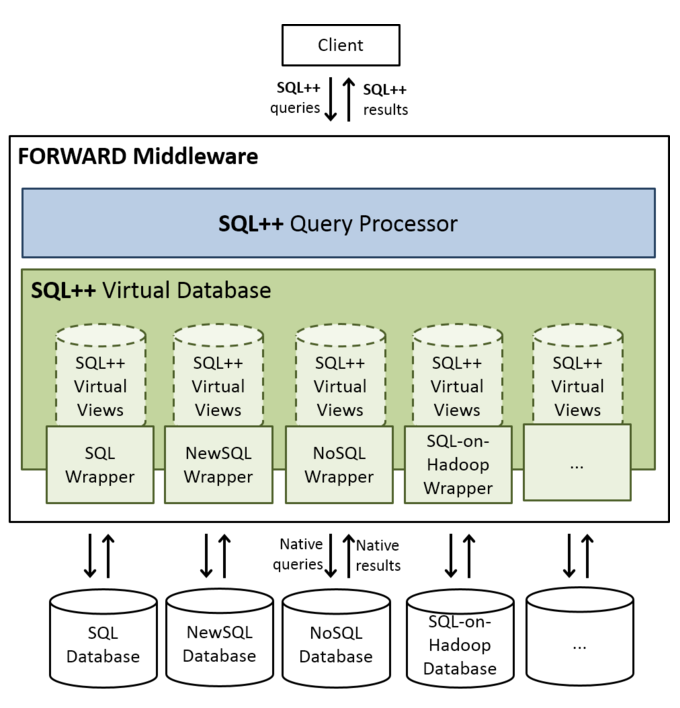
\includegraphics[width=8cm]{images/architecture}
\caption{FORWARD Architecture}
\label{forward}
\end{minipage}\hfill
\end{figure*}

The previous works we have have all tried to improve the performance of the application program expressed using an imperative language. FORWARD \cite{kian-win-ong:2014aa, yupeng-fu:2014aa} presents a completely different approach in which the entire application is expressed declaratively using a single language: SQL++. SQL++ is backwards compatible with SQL while supporting the JSON \cite{JSON} data model, the data model behind many NoSQL applications which also integrates easily with application programming objects. The FORWARD web application framework (see figure \ref{forward}) provides a query processor located on the application server, which can derive multiple execution plans for a given SQL++ query, and pick the one with the smallest cost, the same way a cost-based database query optimizer would, but in a distributed environment.

FORWARD allows the developer to write the running example using a page query (see figure \ref{fig:forward-code}), in which both the data access code and the visualization code are represented. The SQL++ query language is \emph{distributed}, with data being accessed both from the application and the database(s) being seamlessly integrated.  For example, on figure\ref{fig:forward-code}, data is being accessed on line 3 from the database, and on line 8 from the HTTP browser session of the user currently browsing the page. The semantics of the \texttt{fstmt:for} statement (lines 11-16) are to evaluate the query in the \texttt{fstmt:with} clause and output its body for every record in the query's response.

The FORWARD engine is a middleware installed on the application server which includes a query processor which evaluates queries based on a number of virtual views, each view corresponding to data located either on locally (on the application server, for example the HTTP session), or externally in a database. The FORWARD query processor operates in 5 stages :

\begin{figure*}[h]
\centering
\begin{minipage}{0.45\textwidth}
\centering
\begin{SQL}[basicstyle=\small, language=HTML]
SELECT SN.name, sum(O.total_price)
FROM (
  SELECT *
  FROM Nations N
  WHERE N.nation_key IN (4,5,8)
) SN
LEFT OUTER JOIN Customers C
JOIN Orders O 
ON O.cust_ref = C.cust_key
ON C.nation_ref = SN.nation_key
GROUP BY SN.name;
\end{SQL}
\caption{Query sent by FORWARD middleware to database}
\label{fig:forward-query}
\end{minipage} \hfill
\begin{minipage}{0.45\textwidth}
\centering
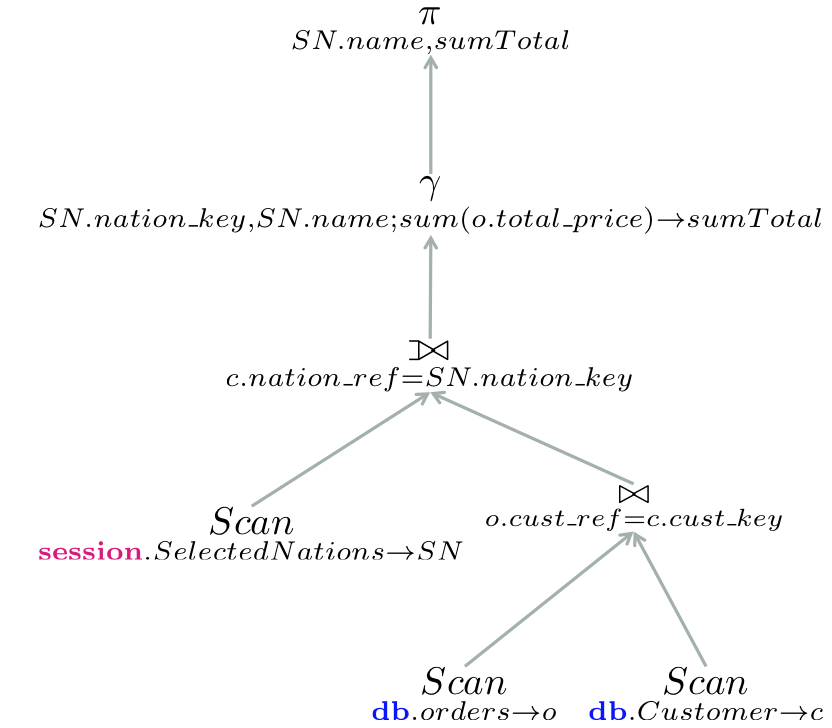
\includegraphics[width=8cm]{images/distributed-plan}
\caption{Distributed Execution Plan}
\label{fig:distributed}
\end{minipage} \hfill
\end{figure*}

\begin{enumerate}
\item{\emph{Syntax Analysis}: the SQL++ queries are parsed into an abstract syntax tree (AST).}
\item{\emph{Initial plan translation \& Source Agnostic Rewritings}: the AST is then converted into a logical plan which is then optimized using source-agnostic rewriting rules. The set-at-a-time execution plan rewriting is a source agnostic rewriting which would be executed at this step. In our running example, the execution plan at this step would be correspond to the set-at-a-time execution plan shown on figure \ref{fig:distributed}. Notice that this plan is distributed, with \texttt{session} and \texttt{db} annotations indicating that the relation is application-resident and database-resident, respectively.}
\item{\emph{Plan Distribution \& Source Specific Rewritings}: The query processor decides where each operation will be computed. In our running example, the query processor will realize that the most efficient execution should ship the data from the \texttt{selectedNations} relation to the \texttt{db} database, and execute the set-at-time join there.}
\item{\emph{Physical Plan Generation \& Native Query Generation}: The distributed query plan is converted into the SQL query shown on figure \ref{fig:forward-query}. Notice that the query exhibits the set-at-a-time execution pattern and sends over the values (4,5,8), which corresponds to the \texttt{nation\_key} attributes of the nations currently selected by the user. }
\item{\emph{Plan Execution}: The generated query is sent to the \texttt{db} database, the results are retrieved by FORWARD and then used to populate the page.}
\end{enumerate}

Note that the distributed query execution and optimization is only one of FORWARD's characteristics. FORWARD also uses incremental view maintenance \cite{fu:2011aa}, to ensure that whenever a collection is updated either on the browser session or on one of the database instances, the change is reflected on the user's browser. 